\chapter{Proposed Manual Evaluation Method}

The method we propose consists of two parts. The first part is a way how humans
judge outputs of judged systems. The second part is how to interpret collected
judgments to compute overall scores and rank the systems. We discuss the first
part in in the following sections. The second part is described in the
subsection \ref{evaluating-annotated-systems}.  \XXX{Tady to asi nejak hodne
predelat} \XXX{V tomto odstavci (a asi i v dalsich odstavcich neni dostatecne
    zdurazneno, proc je to semi-automaticka metoda, mozna opustit oznaceni
semi-automaticka a pouzit misto toho neco jako Manual Evaluation Method with
posibility to reuse collected judgementes for new systems)}



\section{Annotation of Short Segments}

\XXX{Mozna Ranking Short Segments}

\XXX{Mozna Short Segments Ranking}

In the WMT official human evaluation humans judge whole sentences. They get
five candidate translations of a given source sentence and their task is to
rank these candidates relatively (ties are allowed). One of disadvantages of
this method is that sentences are quite long and therefore quite hard to
remember for judge to compare them. Also when comparing longer sentences there
are much more aspects in which one sentence can be better or worse than second
sentence and therefore it is more difficult for judges to choose the better
candidate. 

\begin{algorithm}
    \begin{algorithmic}[1]
        %\Require{$x$ and $y$ are packed DNA strings of equal length $n$}
        %\Statex
        \Function{ExtractSegments}{$tree, minLength, maxLength$}
            \Let{$leaves$}{$tree.leaves()$}
            \If{$length(leaves) \lte maxLength$}
                \If{$lenth(leaves) \gte minLength$}
                    \State Yield $leaves$
                \EndIf
            \Else
                \For{}
                \EndFor
            \EndIf
        \EndFunction
    \end{algorithmic}
    \caption{XXXX}
    \label{segment:extraction}
\end{algorithm}

To avoid these disadvantages we propose the following method. Instead of
judging whole sentences we extract shorter segments from candidates and give
them to judges to rank them. In order to extract meaningful segments with the
same meaning from all candidates we do the following procedure: First we parse
the source sentence and then we go recursively down the parsed tree and find
nodes which covers source segments with given maximum length (which is a
parameter of this method). This is exactly described in algorithm
\ref{segment:extraction}. Finally we project these extracted source segments to
their counterpart segments in all candidate sentences using an automatic
alignment.  You can find the whole process ilustrated in figure \XXX{nakreslit
obrazek}.  This extraction method is inspired by \perscite{human-in-the-loop}
and by the WMT07 manual evaluation \parcite{wmt-overview-2007}.

In the segment evaluation in \parcite{wmt-overview-2007}, these extracted
segments are only highlighted and shown to judges together with the rest of the
sentence.  Judges are asked to rank the the highlighted segments in the context
of whole sentences.

We use different approach here which is more similar to that used in
\parcite{human-in-the-loop}. We show the extracted segments without any context
and ask judges to rank them. The only additional information provided to
annotators is the whole source sentence with the source segment highlighted.
Judges are told that they can imagine the rest of the sentence in which the
ranked segment fits best. They are instructed to penalize only those segments
for which they cannot imagine any appropriate rest of the sentence.

While we are aware that this approach has some disadvantages (which we
summarize bellow) there is one significant advantage: it is much more likely
that two systems produce the same translation of a short segment then they
would produce the same translation of a whole sentence. Because we do not show
the sentence context to annotators we can merge the equal segment candidates
into one, so the annotators have less candidate segments to rank. This also
allows us to reuse already collected human judgements later to evaluate a new
system which was not in the set of annotated systems (we present this
experiment in the section \ref{evaluating-new-systems}) or to tune parameters
of a system (we present this experiment in the section \ref{tuning-systems}).

\XXX{Sumarizovat nevyhody}

\subsection{Data and Segment Preparation}

We have conducted an annotation experiment using the proposed method. In this
section we describe what data we have used and how we prepare them for the
annotation experiment.

We used English to Czech part of the WMT14 \parcite{wmt14-overview-paper} test
set. We choose this data set to be able to compare experiments' results with
the official WMT14 human evaluation. 

The testset consists of 3003 sentences (68866 tokens). It contains both source
sentences and reference translations. Roughly a half of the sentences was
originally in Czech and was translated by human translators into English. The
second half of the sentences was translated in opposite direction. Besides the
source and reference translations, we also used candidate translations of 10
systems which participated in the WMT14 translation task. All systems are
listed in the table \ref{translation-task-participants}

\begin{table}[h]
  \small
  \begin{center}
    \begin{tabular}{|l|l|l|}
      \hline
      \textbf{ID} & \textbf{Type} & \textbf{Team} \\
      \hline
      \system{cu-depfix} & statistical & \multirow{4}{*}{Charles University, Prague \parcite{tamchyna2014}}  \\
      \system{cu-bojar} & statistical &  \\
      \system{cu-funky} & statistical &  \\
      \system{cu-tecto} & statistical &  \\
      \hline
      \system{uedin-phrase} & statistical &  \multirow{2}{*}{University of Edinburgh \parcite{durrani2014}} \\
      \system{uedin-uncnstr} &  statistical &  \\
      \hline
      \system{commercial-1} & rule-based & \multirow{2}{*}{Commercial machine translation systems} \\
      \system{commercial-2} & rule-based & \\
      \hline
      \system{online-a} & statistical & \multirow{2}{*}{Online statistical machine translation systems} \\
      \system{online-b} & statistical & \\
      \hline
    \end{tabular}
  \end{center}

  \caption[The MT systems which were used in the annotation experiment]{The
  machine translation systems participating in the WMT14 translation task in
  direction English-Czech which were used in the annotation experiment
  \XXX{Zkontrolovat typy nekterych systemu}}

  \label{translation-task-participants}
\end{table}

Source sentences and all candidate translations were tokenized using the script
\script{tokenizer.perl}. Unicode punctuation characters were normalized using
the script \script{replace-unicode-punctuation.perl}. (Both scripts are included
in the Moses toolkit).

The source sentences were parsed using the Stanford lexicalized parser
\XXX{citace}. We used \pojem{englishFactored} model which is distributed with
the parser. (More models were examined and this model gave subjectively the
best segments). \XXX{Tady popsat detailneji, ktere modely jsem zkusil a ze 
to nebylo zase tak subjektivni}

We computed an alignments between the source sentecnes and the candidate
translations using Giza++ \parcite{giza-pp}. Since the alignment algorithm is
unsupervised and the amount of all candidate translations is relatively small
($10 \times 3003$), we introduced more data by concatenating all candidate
translations with Europarl parallel corpus (646 605 sentences, \XXX{citovat})
and with \XXX{Jaky je to korpus?} (197 053 sentences, \XXX{citovat}).  The
concatenated parallel corpus was lowercased before alignment computation. 

We extracted short segments from the parsed source trees using the algorithm
\ref{segment:extraction}. The constant \pojem{min-segment-length} was set to
the value 3 to filter out very short segments which are hard to judge without
context. This also helped to reduce the number of extracted segments to be
annotated. The constant \pojem{max-segment-length} was set to the value 6 so
the extracted segments were not too long to judge and in the same time it was
more likely that two candidate translations of a segment were equal and
therefore there would be less items to rank (our aim was to make annotations as
easy and fast as possible). We have experimented with various settings of these
two constants and the final settings seemed to generate reasonable number of
meaningful segments.

\XXX{Nekde zduraznit, ze to jsou vlastne konstituenty, ale asi ne tady, nekde drive}

From 3003 source sentences, we have extracted 8485 segments of length 3 to 6
tokens. That is \XXX{priblizne} 2.83 segments on a sentence on average. By
projecting the source segments to the candidate sentences using the computed
alignments, we got $10 \times 8485 = 84850$ candidate segments. However, after
the merging of equal segments only 50011 candidate segments left. This is 58.9
\% of the original candidate segments, or in other words, after the merging we
got 5.89 (instead of original 10) candidate segments to be ranked for each
source segment on average. Theese prepared candidate segments were inserted
into the database to be ranked by annotators.

\subsection{Segments Ranking}

We have developed a new annotation application for this annotation
project.\footnote{It would be probably possible to customize and use an
    existing annotation application, for example Appraise
    \parcite{mtm12_appraise}.  However, since the ranking of short segments is
    quite specific it would require a lot of customization. We therefore
decided to develop our own light-weight web application which would suit our
needs perfectly and allow us to optimize efficiency of the annotation.} For
implementation details of this application, please see the chapter
\ref{implementation}.

You can find an example screen shot of this application in figure
\ref{segranks-screenshot}. Annotation instructions were displayed on each
annotation screen. This is an English translation of these instructions:

\begin{quote}
A number of segments are extracted from the annotated sentence. You are shown a
few candidate translations for each of these segments. Your task is to
distinguish the acceptable candidate translations (the meaning of the segment
can be guessed despite a few or more errors) from the unacceptable ones (the
meaning is definitely not possible to guess from the candidate segment). Also
please rank the acceptable candidate translations relatively from the best ones
to the worst ones.  Please, place better candidate translations higher, the
worser ones lower. You can place candidates of the same quality on the same
rank. Please place the unacceptable candidates to the position ``Garbage''

Please note that source segments and their candidate translations are chosen
automatically and does not have to be perfect. Consider them as only
approximate clue. If a candidate segment contains an extra word, which does not
correspond to the source segment but otherwise could be in the translated
sentence you do not have to consider such candidate as worser. If something is
missing in the candidate translation you should consider that as an error.
\end{quote}

Our goal was to make the annotation as efficient and user friendly as possible.
Annotators rank all the source segments of a sentence on a single screen (so
that they have to read the whole source sentence and reference translation only
once). For each annotated segment they see the source sentence repeated with
the annotated segment highlighted. Annotators rank the segment candidates by
drag-and-droping them to appropriate rank positions. When all candidates of all
source segments of a sentence are ranked annotators are allowed to submit the
results to the server.  The web interface has responsive design, so it works
correctly on mobile devices.  The drag-and-drop works also on touch screens.
Annotators were therefore able to rank segments on a tablet.

\begin{figure}
    \begin{center}
        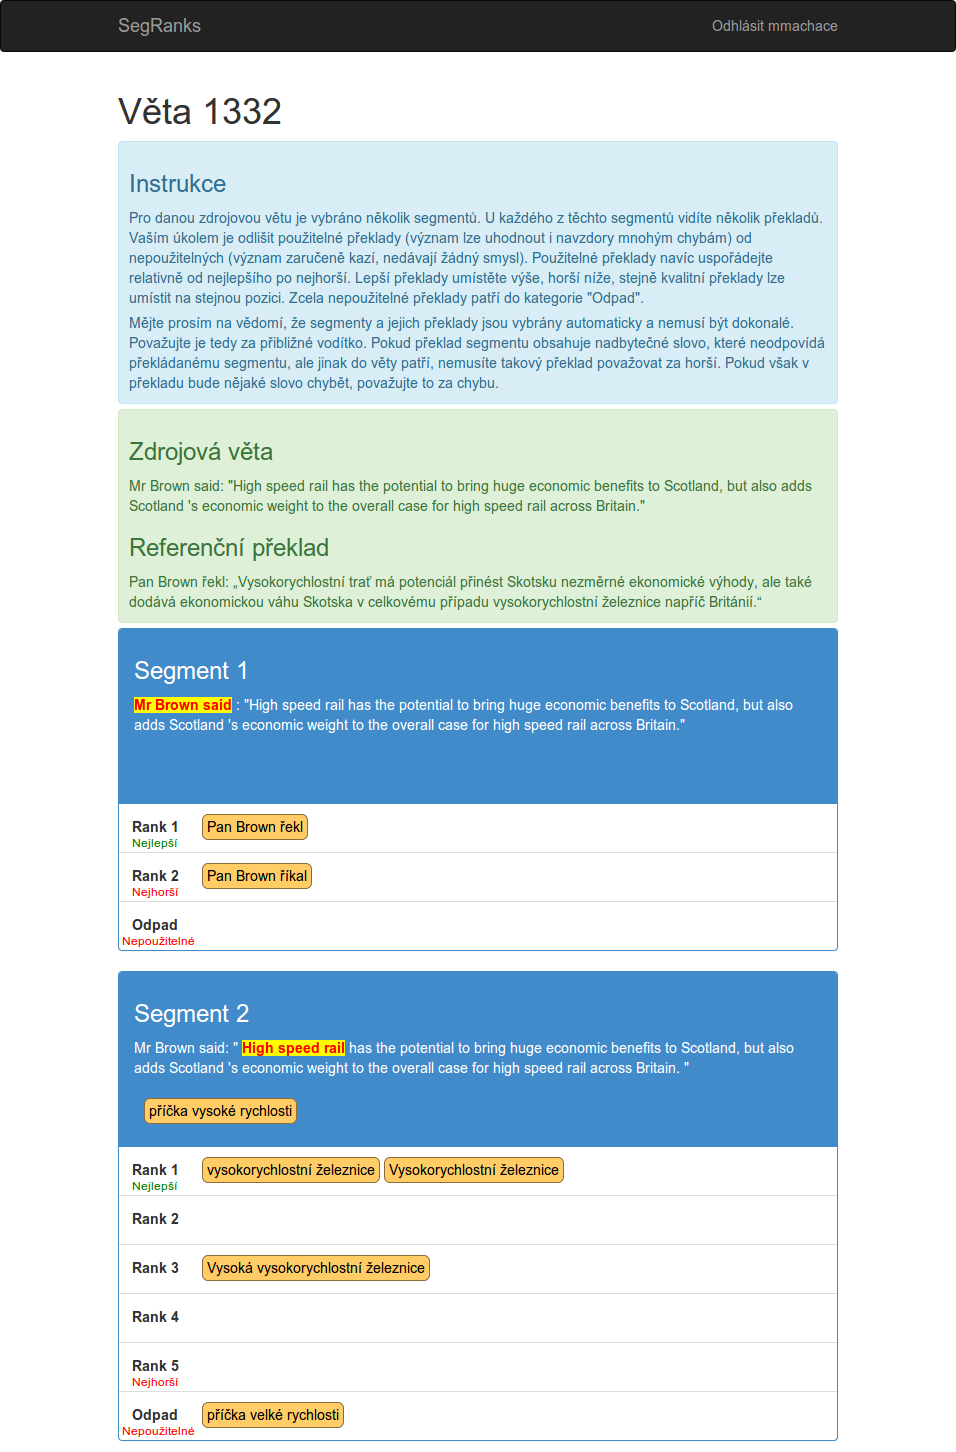
\includegraphics[width=\textwidth]{img/segranks-screenshot2.png}
    \end{center}
    \caption[A screen shot of the annotation application]{A screen shot of the
    annotation application. Annotators rank the candidate segments by dragging
and dropping them into the ranks.  Annotators see all annotated segments of a
sentence on a single screen}
    \label{segranks-screenshot}
\end{figure}

The very annotation experiment was conducted during May/June 2014. It lasted
exactly one month. During this time 17 annotators ranked segments of 2765
sentences, which is more than 92 \% of the prepared English-Czech test set.

\begin{table}
    \begin{center}
        \begin{tabular}{lrrrrrrr}
\textbf{ID} & \rotatebox{90}{\textbf{\#sentences}} & \rotatebox{90}{\textbf{\#segments}} & \textbf{time} & \rotatebox{90}{\textbf{reward/CZK}} & \rotatebox{90}{\textbf{annotatin-time/seconds}} & \rotatebox{90}{\textbf{kappa-intra}} & \rotatebox{90}{\textbf{kappa-inter}} \\
\hline
1 & 78 & 232 & 4:53:43 & 665 & 75 & 0.838 & 0.495 \\
4 & 87 & 248 & 5:00:46 & 711 & 74 & 0.283 & 0.145 \\
6 & 378 & 1160 & 16:53:13 & 3326 & 52 & 0.657 & 0.453 \\
7 & 243 & 663 & 11:16:26 & 1901 & 62 & 0.763 & 0.417 \\
8 & 6 & 20 & 0:21:06 & 57 & 63 \\
9 & 12 & 50 & 0:45:58 & 143 & 55 & 0.686 \\
10 & 98 & 274 & 5:04:45 & 785 & 66 & 0.673 & 0.320 \\
12 & 3 & 7 & 0:15:03 & 20 & 129 & 0.281 \\
13 & 424 & 1260 & 1 day, 2:26:14 & 3613 & 75 & 0.459 & 0.308 \\
15 & 106 & 282 & 5:17:58 & 808 & 67 & 0.611 & 0.401 \\
16 & 224 & 627 & 5:00:11 & 1797 & 28 & 0.655 & 0.614 \\
17 & 26 & 74 & 2:40:44 & 212 & 130 & 0.734 & 0.269 \\
18 & 83 & 234 & 7:02:10 & 670 & 111 & 0.676 & 0.385 \\
19 & 15 & 50 & 1:31:52 & 143 & 110 \\
21 & 483 & 1443 & 1 day, 13:44:37 & 4137 & 94 & 0.663 & 0.383 \\
22 & 117 & 338 & 6:00:36 & 969 & 64 & 0.714 & 0.431 \\
23 & 477 & 1371 & 22:07:35 & 3931 & 58 & 0.376 & 0.363 \\
\hline
   & 2773 & 8333 & 6 days, 14:22:57 & 23895 & 68 & 0.593 & 0.397 \\
        \end{tabular}
    \end{center}

    \caption[The list of annotators and their statistics]{The list of
        annotators and their statistics. The annotators are anonymized using
        their ID. The table contains the number of sentences annodated, the
        number of segments annotated, the time spend annotating, the reward in
    CZK, average time in seconds spend on one segment annotation and
intra-annotator and inter-annotator agreements. }

    \label{big-table}
\end{table}

\subsubsection{Annotator Agreements}

To measure reliability and robustness of the proposed annotation method we have
computed intra- and inter-annotator agreements. \XXX{Neni potreba vysvetlit lepe
co to vlastne je a proc je to potreba?}  We measured the agreements
using the Cohen's kappa coefficient ($\kappa$) \parcite{cohen1960}. Let $P(A)$
be the proportion of times the annotators agree and $P(E)$ be the proportion of
time that they would agree by chance. Then the Cohen's $\kappa$ is computed
using the following formula:

\begin{equation*}
    \kappa = \frac{P(A)-P(E)}{1-P(E)}
\end{equation*}

\noindent Simply put, $\kappa$ is the proportion of times the annotators agrees
from all the times they would not agree by chance. Note that $\kappa$ is a
normalized version of $P(A)$, it considers how difficult it is to agree.
Values of $\kappa$ can be therefore compared across the various annotation
experiments. The maximum value is 1 which means that annotators allways agree.
The zero value means that annotators agree as often as they would by chance.

In our case $P(A)$ and $P(E)$ are computed in context of pairwise comparisons.
Approximately 5 \% of the annotated sentences were annotated twice by two
different annotators (for the inter-annotator agreement).  Another 5 \% of the
sentences were annotated twice by the same annotator (for the intra-annotator
agreement). From all the segments of these double annotated sentences, we
extracted pairwise comparisons of candidate segments. Then we computed $P(A)$
as the proportion of pairwise comparisons in which two annotators agree (or one
annotator in different time in the case of intra-annotator agreement). 

Finally we computed $P(E)$ as 

\begin{equation*}
    P(E) = P(A>B)^2 + P(A=B)^2 + P(A<B)^2
\end{equation*}

\noindent where $P(A>B)$, $P(A=B)$ and $P(A<B)$ were computed empirically. The
value of $P(E)$ in our experiment is 0.394, which means that the probability of
the outcomes $A>B$, $A=B$ and $A<B$ is not uniform.

The final values of inter-annotator and intra-annotator $\kappa$ can be found
in the table \ref{agreements} together with corresponding $\kappa$ values from
WMT14 translation task.  \parcite{wmt14-overview-paper} computed similarly on
the same testset for comparisons. You can see that we get both $\kappa$ scores
better than they are in WMT14. However, they are still quite poor\footnote{ The
exact interpretation of the kappa coefficient is difficult, but according
to \cite{landis77}, 0 -- 0.2 is slight, 0.2 -- 0.4 is fair, 0.4 -- 0.6 is
moderate, 0.6 -- 0.8 is substantial and 0.8 -- 1.0 is almost perfect.} and we
expected them to be higher. We also computed the agreements $\kappa$ for
individual annotators and report them in the table \ref{big-table}.  As you can
see, these scores are varying a lot. Based on these scores we could filter out
unreliable annotators. However we do not do that to have the experiment
comparable to the WMT14 experiment.


\begin{table}
    \begin{center}
        \begin{tabular}{r|cc}
                                     & our method & \cite{wmt14-overview-paper} \\
            \hline
            intra-annotator $\kappa$ &  0.593     & 0.448    \\
            inter-annotator $\kappa$ &  0.397     & 0.360     \\
        \end{tabular}
    \end{center}

    \caption[Inter-annotator and intra-annotator $\kappa$ scores]{$\kappa$
        scores measuring intra-annotator and inter-annotator agreements. We
        also report corresponding $\kappa$ scores from official WMT translation
        task for comparison.  Please see the table \ref{big-table} for the
    annotator agreements computed for individual annotators}

    \label{agreements}
\end{table}




\section{Experiments}

\subsection{Evaluating Annotated Systems}
\label{evaluating-annotated-systems}
\XXX{Zde uvedu vzorecek (mozna vice variant) pro vypocet skore systemu, ktere
byly anotovane. Vypocet skore, vypocet korelace s oficialnimi WMT14 vysledky.
Porovnani obou metod z hlediska mnozstvi lidske prace.}

\subsection{Evaluating New Systems}
\label{evaluating-new-systems}

\XXX{Zde zkusim pouzit vytvorenou databazi pro vyhodnoceni noveho systemu}

\XXX{provest experimenty podobne tem z clanku An Evaluation Tool for Machine
Translation: Fast Evaluation for MT Research}

\subsection{Tuning Systems}
\label{tuning-systems}

\XXX{Zde zkusim pouzit vytvorenou databazi pro MT tuning}

\section{Comparison to Other Manual Methods}
